% ==============================================================================
% Proyecto:     SHRV32 (Space-Hardened RISC-V 32)
% Archivo:      docs/arch/diagram.tex
% Descripción:  Diagrama de bloques de la arquitectura base del SoC (Hito 0)
%               Colores xcolor estándar y coordenadas centradas para Oleafly
% Compilación:  pdflatex diagram.tex  (o copiar tikzpicture en diagram.tikz)
% ==============================================================================
\documentclass[tikz,border=14pt]{standalone}

\usepackage[utf8]{inputenc}
\usepackage[T1]{fontenc}
\usepackage{helvet}
\renewcommand{\familydefault}{\sfdefault}

\usepackage{tikz}
\usetikzlibrary{arrows.meta}

\begin{document}
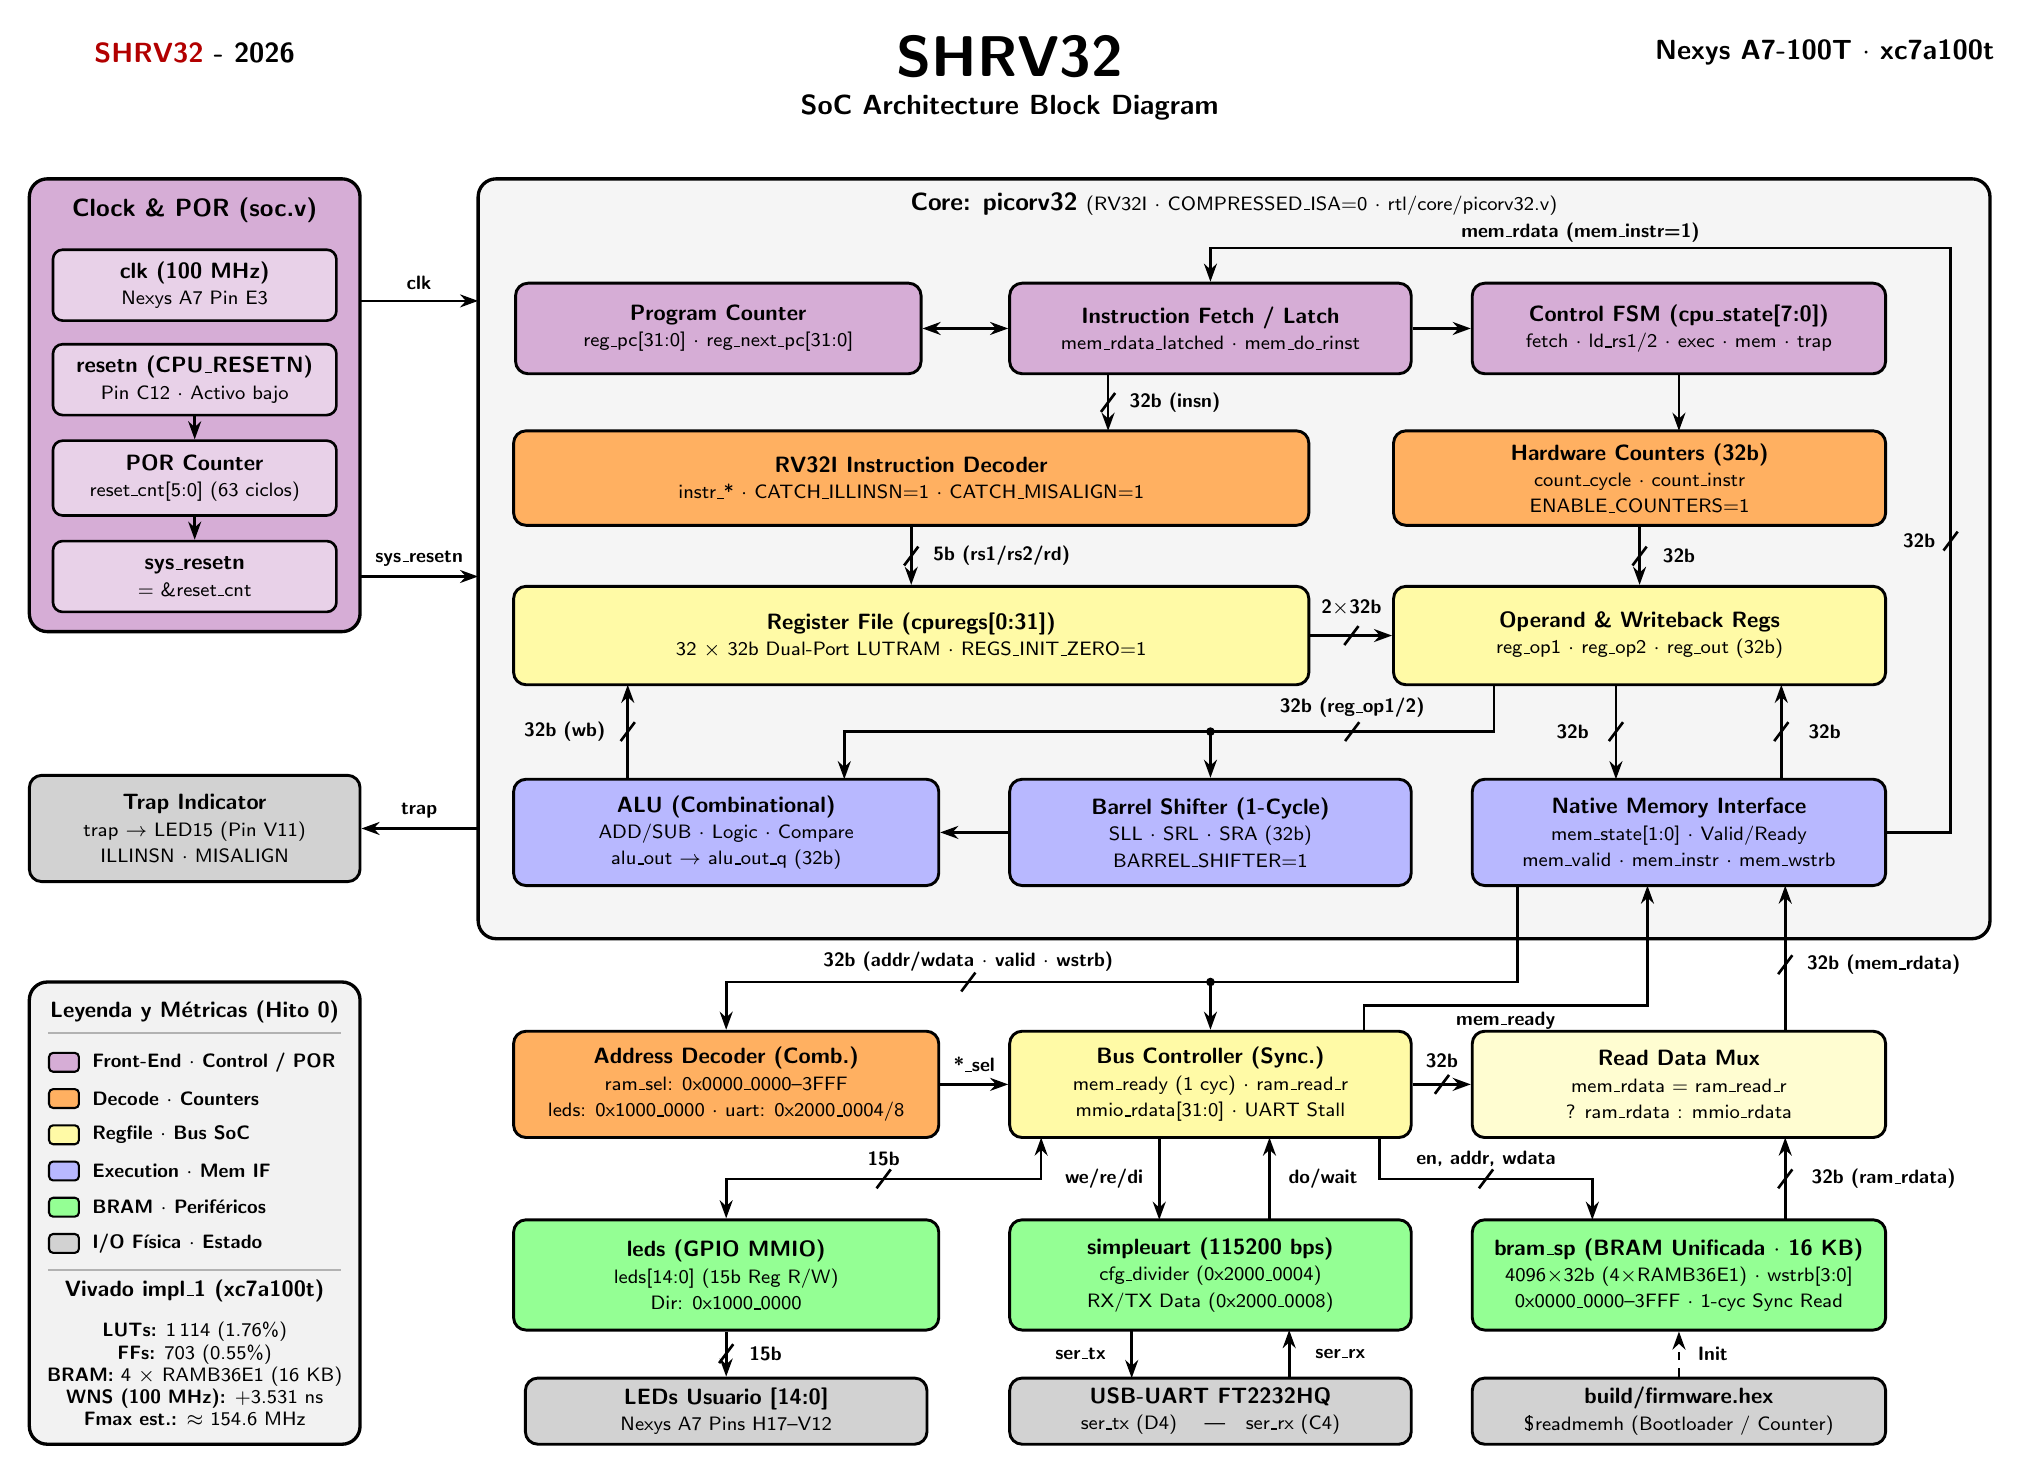
\begin{tikzpicture}[
  >= {Stealth[length=2.3mm, width=1.65mm]},
  blk/.style={
    draw=black,
    line width=1.05pt,
    rounded corners=4.5pt,
    align=center,
    text=black,
    font=\footnotesize,
    inner xsep=4pt,
    inner ysep=3pt
  },
  subblk/.style={
    draw=black,
    line width=0.95pt,
    rounded corners=3.5pt,
    align=center,
    text=black,
    font=\footnotesize,
    inner xsep=4pt,
    inner ysep=2.5pt
  },
  container/.style={
    draw=black,
    line width=1.2pt,
    rounded corners=6.5pt,
    inner sep=0pt
  },
  swatch/.style={
    draw=black,
    line width=0.75pt,
    rounded corners=1.5pt,
    inner sep=0pt,
    minimum width=0.38cm,
    minimum height=0.24cm
  },
  sig/.style={
    ->,
    draw=black,
    line width=0.95pt
  },
  bisig/.style={
    <->,
    draw=black,
    line width=0.95pt
  },
  tick/.style={
    draw=black,
    line width=0.95pt
  },
  lbl/.style={
    font=\scriptsize\bfseries,
    text=black,
    inner sep=1.5pt
  }
]

% ==============================================================================
% 0. Cabecera
% ==============================================================================
\node[font=\normalsize\bfseries] at (2.10, 18.00)
  {\textcolor{red!70!black}{SHRV32} - 2026};
\node[font=\huge\bfseries] at (12.45, 17.95)
  {SHRV32};
\node[font=\normalsize\bfseries] at (12.45, 17.30)
  {SoC Architecture Block Diagram};
\node[font=\normalsize\bfseries] at (22.80, 18.00)
  {Nexys A7-100T $\cdot$ xc7a100t};

% ==============================================================================
% 1. Columna Izquierda: Clock & POR + Trap + Leyenda / Métricas
% ==============================================================================

% --- Contenedor Clock & Power-On Reset (soc.v) ---
\node[container, fill=violet!32, minimum width=4.20cm, minimum height=5.75cm]
  (clk_por_box) at (2.10, 13.525) {};
\node[font=\small\bfseries] at (2.10, 16.00)
  {Clock \& POR (soc.v)};

\node[subblk, fill=violet!18, minimum width=3.60cm, minimum height=0.90cm]
  (clk_in) at (2.10, 15.05)
  {\textbf{clk (100 MHz)}\\\scriptsize Nexys A7 Pin E3};

\node[subblk, fill=violet!18, minimum width=3.60cm, minimum height=0.90cm]
  (rst_in) at (2.10, 13.85)
  {\textbf{resetn (CPU\_RESETN)}\\\scriptsize Pin C12 $\cdot$ Activo bajo};

\node[subblk, fill=violet!18, minimum width=3.60cm, minimum height=0.95cm]
  (por_cnt) at (2.10, 12.60)
  {\textbf{POR Counter}\\\scriptsize reset\_cnt[5:0] (63 ciclos)};

\node[subblk, fill=violet!18, minimum width=3.60cm, minimum height=0.90cm]
  (sys_rst) at (2.10, 11.35)
  {\textbf{sys\_resetn}\\\scriptsize = \&reset\_cnt};

\draw[sig] (rst_in.south) -- (por_cnt.north);
\draw[sig] (por_cnt.south) -- (sys_rst.north);

% --- Indicador de Trampa (LED15) ---
\node[blk, fill=gray!35, minimum width=4.20cm, minimum height=1.35cm]
  (trap_blk) at (2.10, 8.15)
  {\textbf{Trap Indicator}\\\scriptsize trap $\rightarrow$ LED15 (Pin V11)\\\scriptsize ILLINSN $\cdot$ MISALIGN};

% --- Leyenda de Niveles y Métricas Base (Vivado impl_1) ---
\node[container, fill=gray!10, minimum width=4.20cm, minimum height=5.87cm]
  (leyenda_box) at (2.10, 3.265) {};
\node[font=\footnotesize\bfseries] at (2.10, 5.82)
  {Leyenda y Métricas (Hito 0)};
\draw[line width=0.6pt, gray!60] (0.24, 5.55) -- (3.96, 5.55);

\node[swatch, fill=violet!32] (sw_fe) at (0.44, 5.18) {};
\node[font=\scriptsize\bfseries, text width=3.20cm, align=left] at (2.40, 5.18) {Front-End $\cdot$ Control / POR};

\node[swatch, fill=orange!62] (sw_dec) at (0.44, 4.72) {};
\node[font=\scriptsize\bfseries, text width=3.20cm, align=left] at (2.40, 4.72) {Decode $\cdot$ Counters};

\node[swatch, fill=yellow!35] (sw_bus) at (0.44, 4.26) {};
\node[font=\scriptsize\bfseries, text width=3.20cm, align=left] at (2.40, 4.26) {Regfile $\cdot$ Bus SoC};

\node[swatch, fill=blue!28] (sw_exec) at (0.44, 3.80) {};
\node[font=\scriptsize\bfseries, text width=3.20cm, align=left] at (2.40, 3.80) {Execution $\cdot$ Mem IF};

\node[swatch, fill=green!42] (sw_mem) at (0.44, 3.34) {};
\node[font=\scriptsize\bfseries, text width=3.20cm, align=left] at (2.40, 3.34) {BRAM $\cdot$ Periféricos};

\node[swatch, fill=gray!35] (sw_io) at (0.44, 2.88) {};
\node[font=\scriptsize\bfseries, text width=3.20cm, align=left] at (2.40, 2.88) {I/O Física $\cdot$ Estado};

\draw[line width=0.6pt, gray!60] (0.24, 2.54) -- (3.96, 2.54);
\node[font=\footnotesize\bfseries] at (2.10, 2.28)
  {Vivado impl\_1 (xc7a100t)};
\node[align=center, font=\scriptsize] at (2.10, 1.22)
  {\textbf{LUTs:} 1\,114 (1.76\%)\\
   \textbf{FFs:} 703 (0.55\%)\\
   \textbf{BRAM:} 4 $\times$ RAMB36E1 (16 KB)\\
   \textbf{WNS (100 MHz):} +3.531 ns\\
   \textbf{Fmax est.:} $\approx$ 154.6 MHz};

% ==============================================================================
% 2. Núcleo PicoRV32 (rtl/core/picorv32.v)
% ==============================================================================
\node[container, fill=gray!8, minimum width=19.20cm, minimum height=9.65cm]
  (core_box) at (15.30, 11.575) {};
\node[font=\small] at (15.30, 16.08)
  {\textbf{Core: picorv32} \scriptsize (RV32I $\cdot$ COMPRESSED\_ISA=0 $\cdot$ rtl/core/picorv32.v)};

% --- Nivel A: Front-End & Control (Morado) ---
\node[blk, fill=violet!32, minimum width=5.15cm, minimum height=1.15cm]
  (pc_unit) at (8.75, 14.50)
  {\textbf{Program Counter}\\\scriptsize reg\_pc[31:0] $\cdot$ reg\_next\_pc[31:0]};

\node[blk, fill=violet!32, minimum width=5.10cm, minimum height=1.15cm]
  (fetch_unit) at (15.00, 14.50)
  {\textbf{Instruction Fetch / Latch}\\\scriptsize mem\_rdata\_latched $\cdot$ mem\_do\_rinst};

\node[blk, fill=violet!32, minimum width=5.25cm, minimum height=1.15cm]
  (ctrl_fsm) at (20.95, 14.50)
  {\textbf{Control FSM (cpu\_state[7:0])}\\\scriptsize fetch $\cdot$ ld\_rs1/2 $\cdot$ exec $\cdot$ mem $\cdot$ trap};

% --- Nivel B: Decode & Counters (Naranja) ---
\node[blk, fill=orange!62, minimum width=10.10cm, minimum height=1.20cm]
  (decoder) at (11.20, 12.60)
  {\textbf{RV32I Instruction Decoder}\\\scriptsize instr\_* $\cdot$ CATCH\_ILLINSN=1 $\cdot$ CATCH\_MISALIGN=1};

\node[blk, fill=orange!62, minimum width=6.25cm, minimum height=1.20cm]
  (counters) at (20.45, 12.60)
  {\textbf{Hardware Counters (32b)}\\\scriptsize count\_cycle $\cdot$ count\_instr\\\scriptsize ENABLE\_COUNTERS=1};

% --- Nivel C: Register File & Operands (Amarillo) ---
\node[blk, fill=yellow!35, minimum width=10.10cm, minimum height=1.25cm]
  (regfile) at (11.20, 10.60)
  {\textbf{Register File (cpuregs[0:31])}\\\scriptsize 32 $\times$ 32b Dual-Port LUTRAM $\cdot$ REGS\_INIT\_ZERO=1};

\node[blk, fill=yellow!35, minimum width=6.25cm, minimum height=1.25cm]
  (op_regs) at (20.45, 10.60)
  {\textbf{Operand \& Writeback Regs}\\\scriptsize reg\_op1 $\cdot$ reg\_op2 $\cdot$ reg\_out (32b)};

% --- Nivel D: Execution & Memory Interface (Azul) ---
\node[blk, fill=blue!28, minimum width=5.40cm, minimum height=1.35cm]
  (alu) at (8.85, 8.10)
  {\textbf{ALU (Combinational)}\\\scriptsize ADD/SUB $\cdot$ Logic $\cdot$ Compare\\\scriptsize alu\_out $\rightarrow$ alu\_out\_q (32b)};

\node[blk, fill=blue!28, minimum width=5.10cm, minimum height=1.35cm]
  (shifter) at (15.00, 8.10)
  {\textbf{Barrel Shifter (1-Cycle)}\\\scriptsize SLL $\cdot$ SRL $\cdot$ SRA (32b)\\\scriptsize BARREL\_SHIFTER=1};

\node[blk, fill=blue!28, minimum width=5.25cm, minimum height=1.35cm]
  (mem_if) at (20.95, 8.10)
  {\textbf{Native Memory Interface}\\\scriptsize mem\_state[1:0] $\cdot$ Valid/Ready\\\scriptsize mem\_valid $\cdot$ mem\_instr $\cdot$ mem\_wstrb};

% --- Conexiones internas de picorv32 ---
\draw[bisig] (pc_unit.east) -- (fetch_unit.west);
\draw[sig] (fetch_unit.east) -- (ctrl_fsm.west);

\draw[sig] (13.70, 13.925) -- (13.70, 13.20);
\draw[tick] (13.61, 13.44) -- (13.79, 13.68);
\node[lbl] at (14.55, 13.56) {32b (insn)};

\draw[sig] (20.95, 13.925) -- (20.95, 13.20);

\draw[sig] (decoder.south) -- (regfile.north);
\draw[tick] (11.11, 11.49) -- (11.29, 11.73);
\node[lbl] at (12.35, 11.61) {5b (rs1/rs2/rd)};

\draw[sig] (counters.south) -- (op_regs.north);
\draw[tick] (20.36, 11.49) -- (20.54, 11.73);
\node[lbl] at (20.95, 11.61) {32b};

\draw[sig] (regfile.east) -- (op_regs.west);
\draw[tick] (16.70, 10.48) -- (16.88, 10.72);
\node[lbl] at (16.79, 10.95) {2$\times$32b};

% Operandos -> ALU y Barrel Shifter
\draw[sig] (18.60, 9.975) -- (18.60, 9.38) -- (10.35, 9.38) -- (10.35, 8.775);
\draw[sig] (15.00, 9.38) -- (shifter.north);
\fill[black] (15.00, 9.38) circle (0.055);
\draw[tick] (16.71, 9.26) -- (16.89, 9.50);
\node[lbl] at (16.80, 9.68) {32b (reg\_op1/2)};

% Shifter -> ALU y ALU writeback -> Regfile
\draw[sig] (shifter.west) -- (alu.east);
\draw[sig] (7.60, 8.775) -- (7.60, 9.975);
\draw[tick] (7.51, 9.26) -- (7.69, 9.50);
\node[lbl] at (6.80, 9.38) {32b (wb)};

% Operandos / Carga <-> Interfaz de memoria
\draw[sig] (20.15, 9.975) -- (20.15, 8.775);
\draw[tick] (20.06, 9.26) -- (20.24, 9.50);
\node[lbl] at (19.60, 9.38) {32b};

\draw[sig] (22.25, 8.775) -- (22.25, 9.975);
\draw[tick] (22.16, 9.26) -- (22.34, 9.50);
\node[lbl] at (22.80, 9.38) {32b};

% Retorno de instrucción capturada (mem_instr) hacia Fetch
\draw[sig] (mem_if.east) -- (24.40, 8.10) -- (24.40, 15.52) -- (15.00, 15.52) -- (fetch_unit.north);
\draw[tick] (24.31, 11.68) -- (24.49, 11.92);
\node[lbl] at (24.00, 11.80) {32b};
\node[lbl] at (19.70, 15.72) {mem\_rdata (mem\_instr=1)};

% --- Conexiones Core <-> Columna Izquierda ---
\draw[sig] (4.20, 14.85) -- (5.70, 14.85);
\node[lbl] at (4.95, 15.08) {clk};

\draw[sig] (4.20, 11.35) -- (5.70, 11.35);
\node[lbl] at (4.95, 11.58) {sys\_resetn};

\draw[sig] (5.70, 8.15) -- (trap_blk.east);
\node[lbl] at (4.95, 8.38) {trap};

% ==============================================================================
% 3. Nivel E: Bus Nativo SoC y Decodificador de Direcciones (soc.v)
% ==============================================================================
\node[blk, fill=orange!62, minimum width=5.40cm, minimum height=1.35cm]
  (addr_dec) at (8.85, 4.90)
  {\textbf{Address Decoder (Comb.)}\\\scriptsize ram\_sel: 0x0000\_0000--3FFF\\\scriptsize leds: 0x1000\_0000 $\cdot$ uart: 0x2000\_0004/8};

\node[blk, fill=yellow!35, minimum width=5.10cm, minimum height=1.35cm]
  (bus_ctrl) at (15.00, 4.90)
  {\textbf{Bus Controller (Sync.)}\\\scriptsize mem\_ready (1 cyc) $\cdot$ ram\_read\_r\\\scriptsize mmio\_rdata[31:0] $\cdot$ UART Stall};

\node[blk, fill=yellow!18, minimum width=5.25cm, minimum height=1.35cm]
  (rdata_mux) at (20.95, 4.90)
  {\textbf{Read Data Mux}\\\scriptsize mem\_rdata = ram\_read\_r\\\scriptsize ? ram\_rdata : mmio\_rdata};

% Conexiones Core <-> Nivel E (sin cruces)
\draw[sig] (18.90, 7.425) -- (18.90, 6.20) -- (8.85, 6.20) -- (addr_dec.north);
\draw[sig] (15.00, 6.20) -- (bus_ctrl.north);
\fill[black] (15.00, 6.20) circle (0.055);
\draw[tick] (11.835, 6.08) -- (12.015, 6.32);
\node[lbl] at (11.925, 6.46) {32b (addr/wdata $\cdot$ valid $\cdot$ wstrb)};

\draw[sig] (16.95, 5.575) -- (16.95, 5.90) -- (20.55, 5.90) -- (20.55, 7.425);
\node[lbl] at (18.75, 5.71) {mem\_ready};

\draw[sig] (22.30, 5.575) -- (22.30, 7.425);
\draw[tick] (22.21, 6.30) -- (22.39, 6.54);
\node[lbl] at (23.55, 6.42) {32b (mem\_rdata)};

\draw[sig] (addr_dec.east) -- (bus_ctrl.west);
\node[lbl] at (12.00, 5.15) {*\_sel};

\draw[sig] (bus_ctrl.east) -- (rdata_mux.west);
\draw[tick] (17.85, 4.78) -- (18.03, 5.02);
\node[lbl] at (17.94, 5.20) {32b};

% ==============================================================================
% 4. Nivel F: Memoria y Periféricos MMIO (Verde)
% ==============================================================================
\node[blk, fill=green!42, minimum width=5.40cm, minimum height=1.40cm]
  (leds_blk) at (8.85, 2.48)
  {\textbf{leds (GPIO MMIO)}\\\scriptsize leds[14:0] (15b Reg R/W)\\\scriptsize Dir: 0x1000\_0000};

\node[blk, fill=green!42, minimum width=5.10cm, minimum height=1.40cm]
  (uart_blk) at (15.00, 2.48)
  {\textbf{simpleuart (115200 bps)}\\\scriptsize cfg\_divider (0x2000\_0004)\\\scriptsize RX/TX Data (0x2000\_0008)};

\node[blk, fill=green!42, minimum width=5.25cm, minimum height=1.40cm]
  (bram_blk) at (20.95, 2.48)
  {\textbf{bram\_sp (BRAM Unificada $\cdot$ 16 KB)}\\\scriptsize 4096$\times$32b (4$\times$RAMB36E1) $\cdot$ wstrb[3:0]\\\scriptsize 0x0000\_0000--3FFF $\cdot$ 1-cyc Sync Read};

% Conexiones Nivel E <-> Nivel F (rutas disjuntas, sin cruces)
\draw[bisig] (12.85, 4.225) -- (12.85, 3.70) -- (8.85, 3.70) -- (leds_blk.north);
\draw[tick] (10.76, 3.58) -- (10.94, 3.82);
\node[lbl] at (10.85, 3.96) {15b};

\draw[sig] (14.35, 4.225) -- (14.35, 3.18);
\node[lbl] at (13.65, 3.70) {we/re/di};
\draw[sig] (15.75, 3.18) -- (15.75, 4.225);
\node[lbl] at (16.43, 3.70) {do/wait};

\draw[sig] (17.15, 4.225) -- (17.15, 3.70) -- (19.85, 3.70) -- (19.85, 3.18);
\draw[tick] (18.41, 3.58) -- (18.59, 3.82);
\node[lbl] at (18.50, 3.96) {en, addr, wdata};

\draw[sig] (22.30, 3.18) -- (22.30, 4.225);
\draw[tick] (22.21, 3.58) -- (22.39, 3.82);
\node[lbl] at (23.55, 3.70) {32b (ram\_rdata)};

% ==============================================================================
% 5. Nivel G: Pines Físicos Nexys A7-100T y Precarga de Firmware (Gris)
% ==============================================================================
\node[blk, fill=gray!35, minimum width=5.10cm, minimum height=0.84cm]
  (pins_leds) at (8.85, 0.75)
  {\textbf{LEDs Usuario [14:0]}\\\scriptsize Nexys A7 Pins H17--V12};

\node[blk, fill=gray!35, minimum width=5.10cm, minimum height=0.84cm]
  (pins_uart) at (15.00, 0.75)
  {\textbf{USB-UART FT2232HQ}\\\scriptsize ser\_tx (D4) \quad|\quad ser\_rx (C4)};

\node[blk, fill=gray!35, minimum width=5.25cm, minimum height=0.84cm]
  (fw_init) at (20.95, 0.75)
  {\textbf{build/firmware.hex}\\\scriptsize \$readmemh (Bootloader / Counter)};

\draw[sig] (leds_blk.south) -- (pins_leds.north);
\draw[tick] (8.76, 1.36) -- (8.94, 1.60);
\node[lbl] at (9.35, 1.48) {15b};

\draw[sig] (14.00, 1.78) -- (14.00, 1.17);
\node[lbl] at (13.35, 1.48) {ser\_tx};
\draw[sig] (16.00, 1.17) -- (16.00, 1.78);
\node[lbl] at (16.65, 1.48) {ser\_rx};

\draw[sig, dashed] (fw_init.north) -- (bram_blk.south);
\node[lbl] at (21.38, 1.48) {Init};

\end{tikzpicture}
\end{document}
